\documentclass[[12pt,twoside]{book}
\usepackage{_my_document_style}
\begin{document}
%
\def\myDummyValue{-999}
\def\myMach{0.65}
\def\myDummyValue{-999}
\def\myAreaWingMTsquared{499.17}
\def\myAreaWingFTsquared{5373.01}
\def\mySpanWingMT{59.7408}
\def\mySpanWingFT{196}
\def\myTaperRatioWing{0.305}
\def\myInducedDragFactorWing{0.9}
\def\myIncidenceWingRAD{0.03491}
\def\myIncidenceWingDEG{2}
\def\mySweepLEWingRAD{0.7330383}
\def\mySweepLEWingDEG{42}
\def\myXsiTmaxWing{0.3}
\def\mySweepTmaxWingRAD{0.6814218}
\def\mySweepTmaxWingDEG{39.04259}
\def\myDihedralWingRAD{0.08727}
\def\myDihedralWingDEG{5}
\def\myAlphaZeroLiftMeanWingRAD{-0.03743}
\def\myAlphaZeroLiftMeanWingDEG{-2.1}
\def\myThicknessOverChordMeanWing{0.12}
\def\myCmZeroMeanWing{-0.0737588}
\def\myCLAlphaMeanWingRAD{6.06584}
\def\myCLAlphaMeanWingDEG{0.10587}
\def\myChordRootWingMT{14.69}
\def\myChordRootWingFT{48.2}
\def\myChordTipWingMT{4.48}
\def\myChordTipWingFT{14.7}
\def\myRootChordWingLongitudinalPlaneMT{12.23}
\def\myRootChordWingLongitudinalPlaneFT{40.13}
\def\myXEquivalentChordLEToApexWingMT{0}
\def\myXEquivalentChordLEToApexWingFT{0}
\def\myXEquivalentChordTEToApexWingMT{12.231}
\def\myXEquivalentChordTEToApexWingFT{40.127}
\def\myEquivalentTaperRatioWing{0.366}
\def\myEquivalentSweepLEWingRAD{0.73304}
\def\myEquivalentSweepLEWingDEG{42}
\def\myEquivalentSweepQuarterChordWingRAD{0.69604}
\def\myEquivalentSweepQuarterChordWingDEG{39.88}
\def\myEquivalentSweepHalfChordWingRAD{0.6566}
\def\myEquivalentSweepHalfChordWingDEG{37.621}
\def\myEquivalentSweepTEWingRAD{0.56999}
\def\myEquivalentSweepTEWingDEG{32.658}
\def\myAspectRatioEquivalentWing{7.15}
\def\myAspectRatioWing{7.15}
\def\myMACWingMT{9.29}
\def\myMACWingFT{30.47}
\def\myXMACLEToApexWingMT{8.25}
\def\myXMACLEToApexWingFT{27.06}
\def\myAlphaZeroLiftWingRAD{-0.025009}
\def\myAlphaZeroLiftWingDEG{-1.433}
\def\myCriticalMachNumberMACWing{0.988}
\def\myCLAlphaAtMACWingRAD{6.08087}
\def\myCLAlphaAtMACWingDEG{0.1061313}
\def\myCLAlphaWingRAD{5.72254}
\def\myCLAlphaWingDEG{0.0998771}
\def\myKPolhamus{100}
\def\myCLAlphaPolhamusWingRAD{4.54711}
\def\myCLAlphaPolhamusWingDEG{0.0793621}
\def\myCmZeroAWing{-0.0737588}
\def\myCmZeroBWing{0.0532358}
\def\myCmZeroWing{-0.02052}
\def\myXMACLEToApexWingMT{8.24866}
\def\myXMACLEToApexWingFT{27.06254}
\def\myXsiACWing{0.53693}
\def\myXACOverChordRootDatcomWing{0.900896}
\def\myRiggingAngleWingRAD{0.03490659}
\def\myRiggingAngleWingDEG{2}
\def\myAreaWingIMTsquared{233.45}
\def\myAreaWingIFTsquared{2512.84}
\def\mySpanWingIMT{19.8423}
\def\mySpanWingIFT{65.0994}
\def\myTaperRatioWingI{0.602}
\def\myAspectRatioWingI{1.687}
\def\myMACWingIMT{12.008}
\def\myMACWingIFT{39.396}
\def\mySweepLEWingIRAD{0.73304}
\def\mySweepLEWingIDEG{42}
\def\mySweepTEWingIRAD{0.3011}
\def\mySweepTEWingIDEG{17.251}
\def\myTwistWingIRAD{0}
\def\myTwistWingIDEG{0}
\def\myAlphaZeroLiftRootWingIRAD{-0.04363}
\def\myAlphaZeroLiftRootWingIDEG{-2.5}
\def\myAlphaZeroLiftTipWingIRAD{-0.04363}
\def\myAlphaZeroLiftTipWingIDEG{-2.5}
\def\myAlphaZeroLiftMeanWingIRAD{-0.04363}
\def\myAlphaZeroLiftMeanWingIDEG{-2.5}
\def\myAlphaZeroLiftWingIRAD{-0.02041}
\def\myAlphaZeroLiftWingIDEG{-1.17}
\def\myThicknessOverChordRootWingI{0.15}
\def\myThicknessOverChordTipWingI{0.12}
\def\myThicknessOverChordMeanWingI{0.136}
\def\myCmZeroRootWingI{-0.08}
\def\myCmZeroTipWingI{-0.08}
\def\myCmZeroMeanWingI{-0.08}
\def\myCLAlphaRootWingIRAD{6.15}
\def\myCLAlphaRootWingIDEG{0.1073377}
\def\myCLAlphaTipWingIRAD{6.05}
\def\myCLAlphaTipWingIDEG{0.1055924}
\def\myCLAlphaMeanWingIRAD{6.1041451}
\def\myCLAlphaMeanWingIDEG{0.1065374}
\def\myCLAlphaAtMACWingIRAD{6.1041451}
\def\myCLAlphaAtMACWingIDEG{0.1065374}
\def\myKPolhamusI{100}
\def\myCLAlphaPolhamusWingIRAD{2.25978}
\def\myCLAlphaPolhamusWingIDEG{0.0394407}
\def\myChordRootWingIMT{14.69}
\def\myChordRootWingIFT{48.2}
\def\myChordTipWingIMT{8.84}
\def\myChordTipWingIFT{29}
\def\myXsiacRootWingI{0.25}
\def\myXsiacTipWingI{0.25}
\def\myCriticalMachNumberRootWingI{0.65}
\def\myCriticalMachNumberTipWingI{0.7}
\def\myXMACLEToApexWingIMT{4.096}
\def\myXMACLEToApexWingIFT{13.439}
\def\myYMACWingIMT{4.549}
\def\myYMACWingIFT{14.926}
\def\myXsiACWingI{0.55486}
\def\myKOneACDatcomWingI{1.220232}
\def\myKTwoACDatcomWingI{0.0075}
\def\myXACOverChordRootDatcomWingI{0.462221}
\def\myCoeffATwistWingIRADMT{0}
\def\myCoeffATwistWingIDEGMT{0}
\def\myCoeffATwistWingIRADFT{0}
\def\myCoeffATwistWingIDEGFT{0}
\def\myCoeffBTwistWingIRAD{0}
\def\myCoeffBTwistWingIDEG{0}
\def\myCoeffAChordWingI{-0.58987}
\def\myCoeffBChordWingIMT{14.69136}
\def\myCoeffBChordWingIFT{48.2}
\def\myCoeffAAeroTwistWingIRADMT{0}
\def\myCoeffAAeroTwistWingIDEGMT{0}
\def\myCoeffAAeroTwistWingIRADFT{0}
\def\myCoeffAAeroTwistWingIDEGFT{0}
\def\myCoeffBAeroTwistWingIRAD{-0.04363}
\def\myCoeffBAeroTwistWingIDEG{-2.5}
\def\myCoeffAPercThicknessWingIMT{-0.003024}
\def\myCoeffAPercThicknessWingIFT{-0.000922}
\def\myCoeffBPercThicknessWingI{0.15}
\def\myCoeffAClalphaWingIRADMT{-0.0100795}
\def\myCoeffAClalphaWingIRADFT{-0.0030722}
\def\myCoeffAClalphaWingIDEGMT{-0.0001759}
\def\myCoeffAClalphaWingIDEGFT{-5.36e-05}
\def\myCoeffBClalphaWingIRAD{6.15}
\def\myCoeffBClalphaWingIDEG{352.369}
\def\myCoeffACmZeroWingIMT{0}
\def\myCoeffACmZeroWingIFT{0}
\def\myCoeffBCmZeroWingI{-0.08}
\def\myCoeffAXsiACWingIMT{0}
\def\myCoeffAXsiACWingIFT{0}
\def\myCoeffBXsiACWingI{0.25}
\def\myCoeffAMachCrWingIMT{0.00504}
\def\myCoeffAMachCrWingIFT{0.001536}
\def\myCoeffBMachCrWingI{0.7}
\def\myAreaWingIIMTsquared{265.72}
\def\myAreaWingIIFTsquared{2860.18}
\def\myAreaWingIIPrimeMTsquared{358.79}
\def\myAreaWingIIPrimeFTsquared{3861.99}
\def\mySpanWingIIMT{39.8985}
\def\mySpanWingIIFT{130.9006}
\def\mySpanWingIIPrimeMT{49.81965}
\def\mySpanWingIIPrimeFT{163.4503}
\def\myAspectRatioWingII{5.991}
\def\myAspectRatioWingIIPrime{6.918}
\def\myMACWingIIMT{6.898}
\def\myMACWingIIFT{22.63}
\def\myMACWingIIPrimeMT{7.545}
\def\myMACWingIIPrimeFT{24.752}
\def\myTaperRatioWingII{0.507}
\def\myTaperRatioWingIIPrime{0.452}
\def\mySweepLEWingIIRAD{0.73304}
\def\mySweepLEWingIIDEG{42}
\def\mySweepTEWingIIRAD{0.59849}
\def\mySweepTEWingIIDEG{34.291}
\def\myTwistWingIIRAD{-0.05236}
\def\myTwistWingIIDEG{-3}
\def\myAlphaZeroLiftRootWingIIRAD{-0.04363}
\def\myAlphaZeroLiftRootWingIIDEG{-2.5}
\def\myAlphaZeroLiftTipWingIIRAD{-0.01745}
\def\myAlphaZeroLiftTipWingIIDEG{-1}
\def\myAlphaZeroLiftMeanWingIIRAD{-0.03197}
\def\myAlphaZeroLiftMeanWingIIDEG{-1.8}
\def\myAlphaZeroLiftWingIIRAD{-0.0046}
\def\myAlphaZeroLiftWingIIDEG{-0.26}
\def\myThicknessOverChordRootWingII{0.12}
\def\myThicknessOverChordTipWingII{0.09}
\def\myThicknessOverChordMeanWingII{0.107}
\def\myCmZeroRootWingII{-0.08}
\def\myCmZeroTipWingII{-0.04}
\def\myCmZeroMeanWingII{-0.0642127}
\def\myCLAlphaRootWingIIRAD{6.05}
\def\myCLAlphaRootWingIIDEG{0.1055924}
\def\myCLAlphaTipWingIIRAD{6.01}
\def\myCLAlphaTipWingIIDEG{0.1048943}
\def\myCLAlphaMeanWingIIRAD{6.03218}
\def\myCLAlphaMeanWingIIDEG{0.1052814}
\def\myCLAlphaAtMACWingIIRAD{5.9604275}
\def\myCLAlphaAtMACWingIIDEG{0.1040291}
\def\myKPolhamusII{100}
\def\myCLAlphaPolhamusWingIIRAD{4.50859}
\def\myCLAlphaPolhamusWingIIDEG{0.0786898}
\def\myChordRootWingIIMT{8.84}
\def\myChordRootWingIIFT{29}
\def\myChordTipWingIIMT{4.48}
\def\myChordTipWingIIFT{14.7}
\def\myXsiacRootWingII{0.25}
\def\myXsiacTipWingII{0.25}
\def\myCriticalMachNumberRootWingII{0.7}
\def\myCriticalMachNumberTipWingII{0.7}
\def\myXMACLEToApexWingIIMT{8.002}
\def\myXMACLEToApexWingIIFT{26.252}
\def\myYMACWingIIMT{8.887}
\def\myYMACWingIIFT{29.156}
\def\myXsiACWingII{0.11269}
\def\myKOneACDatcomWingII{1.311488}
\def\myKTwoACDatcomWingII{1.008142}
\def\myXACOverChordRootDatcomWingII{1.094066}
\def\myCoeffATwistWingIIRADMT{-0.002625}
\def\myCoeffATwistWingIIDEGMT{-0.15038}
\def\myCoeffATwistWingIIRADFT{-0.0008}
\def\myCoeffATwistWingIIDEGFT{-0.0458363}
\def\myCoeffBTwistWingIIRAD{0}
\def\myCoeffBTwistWingIIDEG{0}
\def\myCoeffAChordWingII{-0.21849}
\def\myCoeffBChordWingIIMT{8.8392}
\def\myCoeffBChordWingIIFT{29}
\def\myCoeffAAeroTwistWingIIRADMT{0.001312}
\def\myCoeffAAeroTwistWingIIDEGMT{0.07519}
\def\myCoeffAAeroTwistWingIIRADFT{0.0004}
\def\myCoeffAAeroTwistWingIIDEGFT{0}
\def\myCoeffBAeroTwistWingIIRAD{-0.04363}
\def\myCoeffBAeroTwistWingIIDEG{-2.5}
\def\myCoeffAPercThicknessWingIIMT{-0.001504}
\def\myCoeffAPercThicknessWingIIFT{-0.000458}
\def\myCoeffBPercThicknessWingII{0.12}
\def\myCoeffAClalphaWingIIRADMT{-0.0020051}
\def\myCoeffAClalphaWingIIRADFT{-0.0006112}
\def\myCoeffAClalphaWingIIDEGMT{-3.5e-05}
\def\myCoeffAClalphaWingIIDEGFT{-1.07e-05}
\def\myCoeffBClalphaWingIIRAD{6.05}
\def\myCoeffBClalphaWingIIDEG{346.639}
\def\myCoeffACmZeroWingIIMT{0.0020051}
\def\myCoeffACmZeroWingIIFT{0.0006112}
\def\myCoeffBCmZeroWingII{-0.08}
\def\myCoeffAXsiACWingIIMT{0}
\def\myCoeffAXsiACWingIIFT{0}
\def\myCoeffBXsiACWingII{0.25}
\def\myCoeffAMachCrWingIIMT{0}
\def\myCoeffAMachCrWingIIFT{0}
\def\myCoeffBMachCrWingII{0.7}
\def\myAreaWingCrankedMTsquared{499.17}
\def\myAreaWingCrankedFTsquared{5373.01}
\def\myMACWingCrankedMT{9.28755}
\def\myMACWingCrankedFT{30.47096}
\def\myAspectRatioWingCranked{7.15}
\def\myXMACLEToApexWingCrankedMT{6.17513}
\def\myXMACLEToApexWingCrankedFT{20.2596}
\def\myXXMACLEToApexWingCrankedMT{8.24866}
\def\myXXMACLEToApexWingCrankedFT{27.06254}
\def\myYMACWingCrankedMT{6.85817}
\def\myYMACWingCrankedFT{22.50056}
\def\myYYMACWingCrankedMT{9.16107}
\def\myYYMACWingCrankedFT{30.05599}

\def\myDummyValue{-999}
\def\myISAAirGasConstNMTKGK{287}
\def\myISAAirAdiabaticIndex{1.4}
\def\myISAAirTemperatureSeaLevelK{288.16}
\def\myISAAirDensitySeaLevelKGMTcubed{1.225}
\def\myISAAirDensitySeaLevelSLUGFTcubed{0.0023769}
\def\myAltitudeMT{5000}
\def\myAltitudeFT{16404.2}
\def\myISALapseRateKMT{-0.0065}
\def\myAirDensityKGMTcubed{0.736}
\def\myAirDensitySLUGFTcubed{0.0014282}
\def\myAirDensityRatio{0.6009}
\def\myAirDynamicViscosiyMTSecKG{1.628e-05}
\def\myAirTemperatureK{255.66}
\def\myAirSoundSpeedMTSec{320.50614}
\def\myAirSoundSpeedFTSec{1051.52934}
\def\myReynoldsPerUnitLengthMT{9417900.73633}
\def\myReynoldsPerUnitLengthFT{2870576.144434}
\def\myDummyValue{-999}
\def\myMach{0.65}
\def\myDummyValue{-999}
\def\myFuselageDiameterAtWingLEMT{6.37}
\def\myFuselageDiameterAtWingLEFT{20.9}
\def\myFuselageLengthMT{70.01}
\def\myFuselageLengthFT{229.7}
\def\myMeanFuselageDiameterMT{6.22}
\def\myMeanFuselageDiameterFT{20.4}
\def\myDistanceBetweenNoseWingLEMT{20.73}
\def\myDistanceBetweenNoseWingLEFT{68}
\def\myDistAlongFCLAtMaxPotentialEnergyMT{54.38}
\def\myDistAlongFCLAtMaxPotentialEnergyFT{178.4}
\def\myFuselageSectionAtZeroPotentialEnergyMTsquared{25.88}
\def\myFuselageSectionAtZeroPotentialEnergyFTsquared{278.6}
\def\myFuselageVerticalWidthNearVTMT{4.82}
\def\myFuselageVerticalWidthNearVTFT{15.8}
\def\myFuselageCrossSectionAverageSurfaceMTsquared{26.2}
\def\myFuselageCrossSectionAverageSurfaceFTsquared{281.99}
\def\myFuselageLateralSurfaceMTsquared{436.29}
\def\myFuselageLateralSurfaceFTsquared{4696.16}
\def\myFuselageVerticalWidthAtQuarterFuselageLengthMT{7.92}
\def\myFuselageVerticalWidthAtQuarterFuselageLengthFT{26}
\def\myFuselageVerticalWidthAtThreeQuarterFuselageLengthMT{6}
\def\myFuselageVerticalWidthAtThreeQuarterFuselageLengthFT{19.7}
\def\myMaxFuselageVerticalWidthMT{8.2}
\def\myMaxFuselageVerticalWidthFT{26.9}
\def\myMaxFuselageVerticalWidthFromTopViewMT{6.37}
\def\myMaxFuselageVerticalWidthFromTopViewMT{20.9}
\def\myFuselageFinenessRatio{11.26}
\def\myFuselageMunchMassFactor{0.9399}
\def\myNoStripCMZeroBody{14}
\def\myDxStripCMZeroBodyMT{5.001}
\def\myDxStripCMZeroBodyFT{16.407}
\def\myNoStripForebodyCMAlphaBody{9}
\def\myDxStripForebodyCMAlphaBodyMT{2.303}
\def\myDxStripForebodyCMAlphaBodyFT{7.556}
\def\myNoStripWingCMAlphaBody{4}
\def\myDxStripWingCMAlphaBodyMT{3.673}
\def\myDxStripWingCMAlphaBodyFT{12.05}
\def\myNoStripAfterbodyCMAlphaBody{9}
\def\myDxStripAfterbodyCMAlphaBodyMT{3.844}
\def\myDxStripAfterbodyCMAlphaBodyFT{12.611}
\def\myFuselagePitchingMomentCoefficienAtZeroLift{-0.05358}
\def\myFactorMWHDownwashGradientBody{0}
\def\myFactorRWHDownwashGradientBody{1.13232}
\def\myFactorKARDownwashGradientBody{0.10577}
\def\myFactorKlambdaDownwashGradientBody{1.29787}
\def\myFactorKmrDownwashGradientBody{0.95942}
\def\myDownwashGradientAtMachZeroBody{0.33987}
\def\myDownwashGradientBody{0.25828}
\def\myFuselagePitchingMomentCoefficientGradientRAD{0.60149}
\def\myFuselagePitchingMomentCoefficientGradientDEG{0.01}
\def\myFuselagePitchingMomentCoefficientGradientMulthoppRAD{0.59839}
\def\myFuselagePitchingMomentCoefficientGradientMulthoppDEG{0.01}
\def\myDeltaXsiACWingBody{-0.132}
\def\myDeltaXsiACWingBodyMulthopp{-0.132}
\def\myXsiACWingBody{0.405}
\def\myXsiACWingBodyMulthopp{0.405}
\def\myDummyValue{-999}
\def\myWHTLEHorizontalDistanceMT{38.8}
\def\myWHTLEHorizontalDistanceFT{127.3}
\def\myWHTRootVerticalDistanceMT{3.5}
\def\myWHTRootVerticalDistanceFT{11.48}
\def\myXWingTEToHTailACMT{29.825}
\def\myXWingTEToHTailACFT{97.852}
\def\myMACHTailMT{5.702}
\def\myMACHTailFT{18.7073}
\def\myXMACLEToApexHTailMT{4.29}
\def\myXMACLEToApexHTailFT{14.0748}
\def\myYMACHTailMT{4.442}
\def\myYMACHTailFT{14.5735}
\def\myXWingACToHTailACMT{31.2811}
\def\myXWingACToHTailACFT{102.6283}
\def\myZWingACToHTailACMT{2.9313}
\def\myZWingACToHTailACFT{9.6171}
\def\myXWingMACQuarterChordToHTailMACQuarterChordMT{33.946}
\def\myXWingMACQuarterChordToHTailMACQuarterChordFT{111.3712}
\def\myZWingMACQuarterChordToHTailMACQuarterChordMT{2.9313}
\def\myZWingMACQuarterChordToHTailMACQuarterChordFT{9.6171}
\def\myXrWingMACQuarterChordToHTailMACQuarterChordMT{33.823}
\def\myXrWingMACQuarterChordToHTailMACQuarterChordFT{110.9678}
\def\myZrWingMACQuarterChordToHTailMACQuarterChordMT{4.1142}
\def\myZrWingMACQuarterChordToHTailMACQuarterChordFT{13.4981}
\def\myFactorMWHDownwashGradientHTail{0.13774}
\def\myFactorRWHDownwashGradientHTail{1.13232}
\def\myFactorKARDownwashGradientHTail{0.10577}
\def\myFactorKlambdaDownwashGradientHTail{1.29787}
\def\myFactorKmrDownwashGradientHTail{0.89335}
\def\myDihedralHTailRAD{0.05236}
\def\myDihedralHTailDEG{3}
\def\myXsiacHTail{0.25}

%
\begin{myExampleX}{Aerodynamic characteristics of the fuselage}{\ding{46}}% \ \Keyboard\ %
\label{example:Fuselage:Multhopp:A}
%
\noindent
We want to calculate the coefficients \smash{$C_{\mathcal{M}_\mathlarger{0,\Body}}$}
and \smash{$C_{\mathcal{M}_\mathlarger{\alpha},\Body}$}
of a fuselage with the \emph{Strip Integration Method} of Multhopp.
For this purpose a \emph{Wing-Body} configuration is considered similar to that of a Boeing~747.
%
Here are some of its features that will be used for the fuselage calculations:
\[
\AR=\SI[round-precision=2]{\myAspectRatioWing}{}\;,
\quad
b=\SI[round-precision=2]{\mySpanWingMT}{m}\;,
\quad
S = \SI[round-precision=1]{\myAreaWingMTsquared}{m^2}\;,
\quad
c_\mathrm{r}=\SI[round-precision=1]{\myChordRootWingMT}{m}\;
\quad
\bar{c} = \SI[round-precision=2]{\myMACWingMT}{m}
\]
\[
\alpha_{0L,\Wing} %= \SI[round-precision=4]{\myAlphaZeroLiftWingRAD}{rad}
  =\SI[round-precision=1]{\myAlphaZeroLiftWingDEG}{deg}\;,
\quad
i_\Wing=\SI[round-precision=1]{\myRiggingAngleWingDEG}{deg}\;,
\quad
\lambda\equiv\lambda_\text{eqv}=\SI[round-precision=2]{\myEquivalentTaperRatioWing}{}\;,
\quad
\Lambda_{c/4}\equiv\Lambda_{c/4,\text{eqv}} = \SI[round-precision=1]{\myEquivalentSweepLEWingDEG}{deg}
\]
Furthermore,
the assigned wing has a lift gradient
$C_{L_\mathlarger{\alpha},\Wing}=\SI[round-precision=2]{\myCLAlphaPolhamusWingRAD}{rad^{-1}}=\SI[round-precision=4]{\myCLAlphaPolhamusWingDEG}{deg^{-1}}$.

Regarding the reference operating conditions, in this example we consider a
flight Mach number $M=\SI[round-precision=2]{\myMach}{}$
and a flight altitude $h_\mathrm{ASL}=\SI[round-precision=2]{\myAltitudeMT}{\metre}$.

The side view and the top view of the fuselage are shown in the
figures~\ref{fig:Fuselage:Multhopp:Results:AA:A} e~\ref{fig:Fuselage:Multhopp:Results:AA:B}.
Said $X$ the longitudinal coordinate running aft along
the \emph{Fuselage Reference Line}, FRL,
with origin at the front end, and $Z$ the coordinate normal to it
taken in the plane of symmetry, we recognize:
\begin{compactitem}[{\color{gray}$\circ$}]% needs paralist package
\item
the function $w_\mathrm{f}(X)$, width of the plan view of the fuselage to the station $X$,
\item
the pair of functions
$\big(X_\mathrm{cl,f}(X),Z_\mathrm{cl,f}(X)\big)$, which describe the \emph{camber line} of the side view,
\item
the function $i_\mathrm{cl,f}(X)$,representing the angle, with changed sign, formed
of the local tangent to the mean line with the FRL.
\end{compactitem}

A discretization for fuselage strips --- visually represented in the
figure~\ref{fig:Fuselage:Multhopp:Results:AA} 
with  $N_{\mathrm{f}0}=\num[round-precision=0]{\myNoStripCMZeroBody}$ stripes
whose thick is $\upDelta X=\SI[round-precision=1]{\myDxStripCMZeroBodyMT}{m}$
---
led to the numerical values listed in the table~\ref{tab:Fuselage:Multhopp:Results:A:A}.
In it, for $k=1,\ldots,\num[round-precision=0]{\myNoStripCMZeroBody}$, the coordinates
$\big(X_{\mathrm{cl,f}_\mathlarger{k}},Z_{\mathrm{cl,f}_\mathlarger{k}}\big)$ of the centroids
of each strip, the widths $w_{\mathrm{f}_\mathlarger{k}}$ 
and angles $i_{\mathrm{cl,f}_\mathlarger{k}}$ are observed.

\EnlargedFigureX% needs two latex passes
  {p}% #1: t, b, p
  {%
    \begin{tabular}{@{}c@{}}
    \subfloat[Vista laterale\label{fig:Fuselage:Multhopp:Results:AA:A}]{%
    \makebox[\textwidth][c]{%
      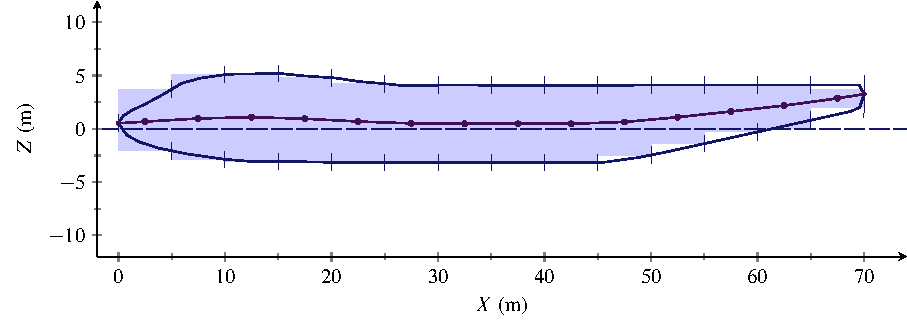
\includegraphics[width=0.90\textwidth]{Chapter_3/aerodynamic_characteristics_of_the_fuselage/fuselage_sideview_1.pdf}%
    }% end-of-makebox
    }% end-of-subfloat
    \\
    \subfloat[Vista dall'alto\label{fig:Fuselage:Multhopp:Results:AA:B}]{%
    \makebox[\textwidth][c]{%
      \rule{2.2mm}{0pt}% --> hack
      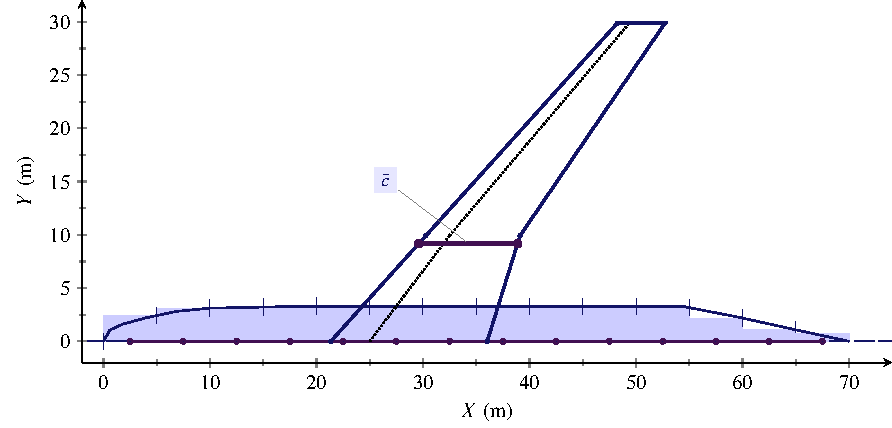
\includegraphics[width=0.88\textwidth]{Chapter_3/aerodynamic_characteristics_of_the_fuselage/fuselage_topview_1.pdf}%
    }% end-of-makebox
    }% end-of-subfloat
    \\
    \subfloat[Incidence of the local tangent to the mean line\label{fig:Fuselage:Multhopp:Results:AA:C}]{%
    \makebox[\textwidth][c]{%
      \rule{3.7mm}{0pt}% --> hack
      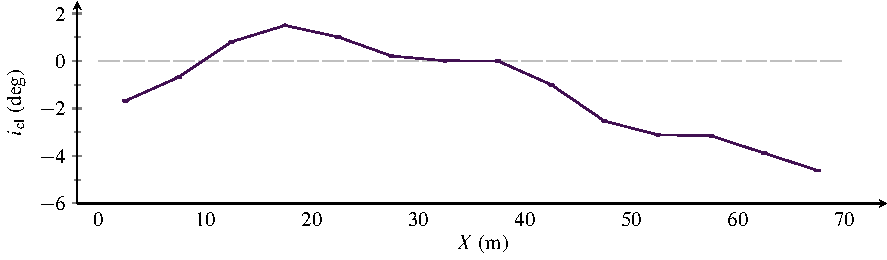
\includegraphics[width=0.895\textwidth]{Chapter_3/aerodynamic_characteristics_of_the_fuselage/fuselage_icl.pdf}%
    }% end-of-makebox
    }% end-of-subfloat
    \end{tabular}
    \vspace{0.3cm}
  }% #2: the image file included by \includegraphics
  {\finalhyphendemerits=100
    Fuselage of a Boeing~747.
    Discretization of the lateral projection for the approximate calculation of the coefficient
    \smash{$C_{\mathcal{M}0,\Body}$}
    with Multhopp's strip integration method.
   Below is the angle $i_\mathrm{cl}$ formed by the local tangent to the \emph{camber line}
   of the fuselage with the FRL.
  }% #3: the caption text
  {fig:Fuselage:Multhopp:Results:AA}%% #4: the label
%
The coefficient of pitching moment due to the fuselage under zero lift conditions
--- that is when $L_{\Wing\Body}=0$ --- is given by the formula
\[
%\begin{equation}\label{eq:Aero:CMBW:Zero}
C_{\mathcal{M}_\mathlarger{0,\Body}} \equiv C_{\mathcal{M}_\mathlarger{0L,\Body(\Wing)}}
    = \frac{\pi}{2}
    \frac{k_2 - k_1}{S \bar{c}}
    %\frac{k_2 - k_1}{\num[round-precision=1]{36.5}\msp S \bar{c}}
      \, \int_{0}^{l_\Body} w_\mathrm{f}^2\msp(X) \,
      \big[\msp i_\Wing -\alpha_{0L,\text{W}} + i_{\mathrm{cl,f\msp}}(X)\msp\big] \diff{X}
%\end{equation}
\]
in which the angles are expressed in \si{rad}.
To evaluate the final result --- being known the following quantities 
$S$, $\bar{c}$, $i_{\Wing}$ e $\alpha_{0L,\Wing}$, related to the wing ---
the laws of $w_\mathrm{f}\msp(X)$ e $i_{\mathrm{cl,f\msp}}(X)$ must be determined 
and the apparent mass coefficient must be calculated $k_2-k_1$.
The latter is derived from the figure~\ref{fig:Fuselage:Munch:Mass:Factor} obtaining
\[
k_2-k_1=\SI[round-precision=2]{\myFuselageMunchMassFactor}{}
\]
corresponding to the \emph{Fuselage Fineness Ratio}, FFR.
% $\text{\itshape FFR}=l_\Body/d_\Body=\SI[round-precision=2]{\myFuselageFinenessRatio}{}$.
$l_\Body/d_\Body=\SI[round-precision=1]{\myFuselageFinenessRatio}{}$.

The calculation formula of the \smash{$C_{\mathcal{M}_\mathlarger{0,\Body}}$} is approximated by substituting for the definite integral
a summation. This approximation is based on the discretization of the aforementioned fuselage shape.
With reference to the values in the table~\ref{tab:Fuselage:Multhopp:Results:A:A} we get
\[
%\begin{equation}\label{eq:Aero:CMBW:Zero}
C_{\mathcal{M}_\mathlarger{0,\Body}} \approx
    \frac{\pi}{2}
    \frac{k_2 - k_1}{S \bar{c}} \,
    %\frac{k_2 - k_1}{\num[round-precision=1]{36.5}\msp S \bar{c}}
      \sum_{k=1}^{\num[round-precision=0]{\myNoStripCMZeroBody}} 
        w_{\mathrm{f}_\mathlarger{k}}^2
        \Big(\msp i_\Wing -\alpha_{0L,\text{W}} + i_{\mathrm{cl,f}_\mathlarger{k}}\msp\Big) \upDelta X
  = 
    \mathunderline{mydarkblue}{ 
      \SI[round-precision=4]{\myFuselagePitchingMomentCoefficienAtZeroLift}{} 
    }
%\end{equation}
\]

As can be understood from the side view of the fuselage and from the trend of the midline
--- see the sequence diagram $\big(X_{\mathrm{cl,f}_\mathlarger{k}},i_{\mathrm{cl,f}_\mathlarger{k}}\big)$ 
in the figure~\ref{fig:Fuselage:Multhopp:Results:AA:C} --- 
for a flow that cuts at an angle
$-i_\Wing+\alpha_{0L,\Wing}=\calcSI[round-precision=1,fixed-exponent=0,scientific-notation=fixed]{-(\myIncidenceWingDEG)+\myAlphaZeroLiftWingDEG}{deg}$
with respect to the reference line of the fuselage
the pitching moment is descending.
%
\begin{table}[tb]
\caption{%
  Discrete values used in the formula for calculating the coefficient of
   moment \smash{$C_{\mathcal{M}_\mathlarger{0,\Body}}$}.
}
\label{tab:Fuselage:Multhopp:Results:A:A}
\centering
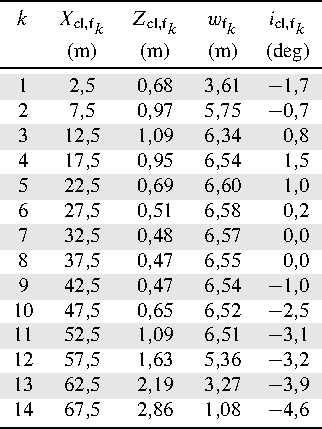
\includegraphics[width=0.38\textwidth]{Chapter_3/aerodynamic_characteristics_of_the_fuselage/fuselage_multhopp_table_1.pdf}
\end{table}
%
\begin{figure}
  [t]%[H]%[!htbp]
  %\centering
  %\checkoddpage
  %\centering
    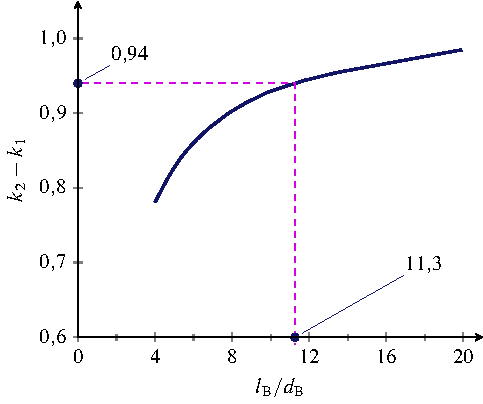
\includegraphics[width=0.58\textwidth]{Chapter_3/aerodynamic_characteristics_of_the_fuselage/fuselage_k2_minus_k1_res.pdf}%
  \caption{\finalhyphendemerits=1000
           Apparent mass coefficiente $k_2-k_1$ of the fuselage
            as a function of the \emph{Fuselage Fineness Ratio}, FFR $l_\Body/d_\Body$ 
          .}
  \label{fig:Fuselage:Munch:Mass:Factor}%
\end{figure}
The focus now shifts to the gradient of the fuselage's pitch moment coefficient.
It is given by the formula
\[
%\begin{equation}\label{eq:Aero:CMBW:Alpha:Multhopp}
C_{\mathcal{M}_\mathlarger{\alpha},\Body} 
  % \equiv \bigg(\frac{\partial \CM}{\partial\alpha}\bigg)_{\!\Body(\Wing)} 
  \equiv \big(C_{\mathcal{M}_\alpha}\big)_{\!\Body(\Wing)} 
  =
    \frac{\pi}{2 S \bar{c}}\, \int_{0}^{l_\Body} w_\mathrm{f}(X)^2 \,
      \bigg(1+\frac{\partial\epsilon_\mathrm{u}(X)}{\partial\alpha}\bigg) \diff{X}
%\end{equation}
\]
where $\epsilon_\mathrm{u}(X)$ is the angle of \emph{upwash}induced by the main lifting surface
to the generic longitudinal station $X$
(note that downstream of the wing $\epsilon_\mathrm{u}=-\epsilon_\mathrm{u}<0$, where \emph{downwash} $\epsilon >0$). 

It is convenient to decompose the integral of the right side into the sum of three integrals.
They will be extended to the front of the fuselage, respectively
(\emph{forebody}), running from the bow to the leading edge of the root chord
of the wing, to the part of the fuselage subtended by the wing root (\emph{wing trunk})
and to the rear of the aircraft(\emph{afterbody}),running from the trailing edge of the root chord
wing up to the stern.
%
\begin{figure} [t]%[H]%[!htbp]
  %\centering
  %\checkoddpage
  %\centering
    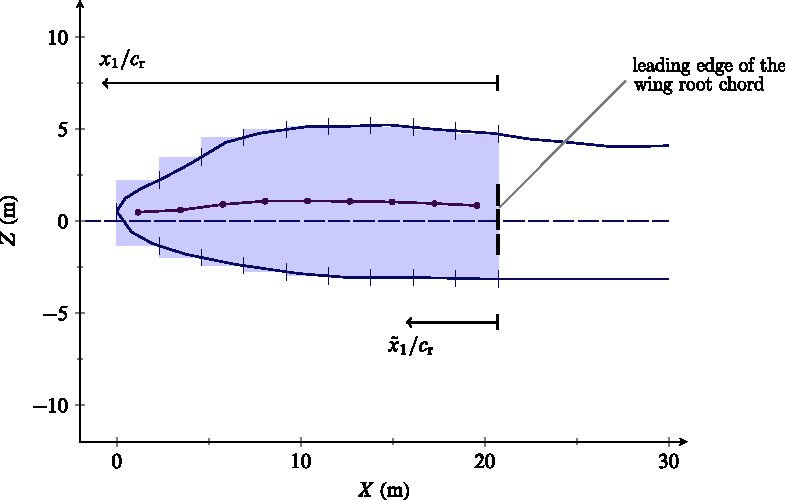
\includegraphics[width=0.88\textwidth]{Chapter_3/aerodynamic_characteristics_of_the_fuselage/fuselage_sideview_1_forebody.pdf}%
  \caption{\finalhyphendemerits=1000
           Side view of the part of the fuselage in front of the leading edge
            of the root chord (\emph{forebody}) and discretization in  
           \num[round-precision=0]{\myNoStripForebodyCMAlphaBody} strips.
           Definition of dimensionless coordinates $\tilde{x}_1/c_\mathrm{r}$
           and $x_1/c_\mathrm{r}$ used in the figure~\ref{fig:Fuselage:Upwash:Gradient}.
  }
  \label{fig:Fuselage:Sideview:Forebody}%
\end{figure}
%
With reference to the figures~\ref{fig:Fuselage:Sideview:Forebody} e~\ref{fig:Fuselage:Sideview:Afterbody}
three new longitudinal coordinates are introduced along the FRL:
\begin{compactitem}[{\color{gray}$\circ$}]% needs paralist package
\item
the coordinate $x_1$ which runs towards the bow and originates at the edge
of attack of the wing root,
\item
the coordinate $x_\Wing$ which runs aft and has the same origin as $x_1$,
\item
the coordinate $x_2$ which runs aft and originates at the trailing edge of the wing root.
\end{compactitem}

The calculation formula of the \smash{$C_{\mathcal{M}_\mathlarger{\alpha},\Body}$} can therefore be rewritten as follows:
\[
%\begin{equation}\label{eq:Aero:CMBW:Alpha:Multhopp}
\begin{split}
C_{\mathcal{M}_\mathlarger{\alpha},\Body} 
  & {}=
    \frac{\pi}{2 S \bar{c}}\, \int\limits_{0}^{l_1} w_\mathrm{f}^2(x_1) \,
      \left[1+\frac{\partial\epsilon_\mathrm{u}(x_1)}{\partial\alpha}\right] \diff{x_1}
  + 
    \frac{\pi}{2 S \bar{c}}\, \int\limits_{0}^{l_\Wing} w_\mathrm{f}^2(x_\Wing) \,
      \left[1+\frac{\partial\epsilon_\mathrm{u}(x_\Wing)}{\partial\alpha}\right] \diff{x_\Wing}
\\[9pt]
  & 
    \rule{5em}{0pt}
    {}+ 
    \frac{\pi}{2 S \bar{c}}\, \int\limits_{0}^{l_3} w^2_\mathrm{f}(x_2) \,
      \left[1+\frac{\partial\epsilon_\mathrm{u}(x_2)}{\partial\alpha}\right] \diff{x_2}
\end{split}
%\end{equation}
\]
where $l_1$, $l_\Wing=c_{\Wing,\mathrm{r}}$ ed $l_2=l_\Body - l_1 - c_{\Wing,\mathrm{r}}$
are the lengths, respectively, of the anterior trunk (\emph{nose}) of the fuselage,
of the central trunk of the fuselage affected by the wing (\emph{wing trunk})
and of the posterior trunk (\emph{tail trunk}).
A significant dimension is the longitudinal distance $l'_\Htail$ 
between the trailing edge of the wing root chord and the aerodynamic center of the horizontal tail.
As shown in the figure~\ref{fig:Fuselage:Sideview:Afterbody}, can be assumed for the aircraft under consideration
\[
l'_\Htail=\SI[round-precision=1]{\myXWingTEToHTailACMT}{m}
\]

%
\EnlargedFigureX% needs two latex passes
  {t}% #1: t, b, p
  {%
    \begin{tabular}{@{}c@{}}
    \makebox[\textwidth][c]{%
      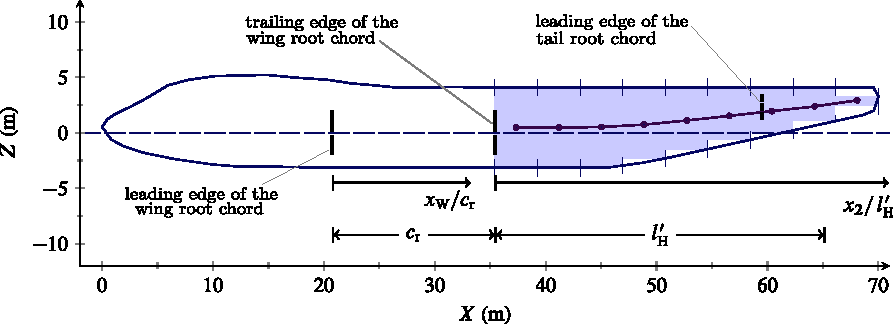
\includegraphics[width=1.00\textwidth]{Chapter_3/aerodynamic_characteristics_of_the_fuselage/fuselage_sideview_1_afterbody.pdf}%
    }% end-of-makebox
    \end{tabular}
    %\vspace{0.3cm}
  }% #2: the image file included by \includegraphics
  {\finalhyphendemerits=1000
           Discretization of the fuselage downstream of the trailing edge
            of the wing root chord (\emph{afterbody}).
           Definition of dimensionless coordinates $x_\Wing/c_\mathrm{r}$ and $x_2/l'_\Htail$, with
           $c_\mathrm{r}=\SI[round-precision=1]{\myChordRootWingMT}{m}$ and
           $l'_\Htail=\SI[round-precision=1]{\myXWingTEToHTailACMT}{m}$.
  }% #3: the caption text
  {fig:Fuselage:Sideview:Afterbody}%% #4: the label
%
%
The second integral to the second member of the above formula can be overlooked
compared to the other two in the sense that the central trunk of the fuselage does not contribute in
significantly to the final result.
Therefore, we obtain the formula
\[
%\begin{equation}\label{eq:Aero:CMBW:Alpha:Multhopp}
C_{\mathcal{M}_\mathlarger{\alpha},\Body} 
  \simeq
    \frac{\pi}{2 S \bar{c}}\, \int\limits_{0}^{l_1} w_\mathrm{f}^2(x_1) \,
      \left[1+\frac{\partial\epsilon_\mathrm{u}(x_1)}{\partial\alpha}\right] \diff{x_1}
  + 
    \frac{\pi}{2 S \bar{c}}\, \int\limits_{0}^{l_2} w_\mathrm{f}^2(x_2) \,
      \left[1+\frac{\partial\epsilon_\mathrm{u}(x_2)}{\partial\alpha}\right] \diff{x_2}
%\end{equation}
\]

The previous result can be approximated by substituting integrals for summations
after having appropriately discretized the front and rear parts of the fuselage.
An example of discretization is given by the figure~\ref{fig:Fuselage:Sideview:Forebody} e~\ref{fig:Fuselage:Sideview:Afterbody}.
The three fuselage trunks--- front, middle and rear --- are divided,
respectively, in
$N_{\mathrm{f}1}=\num[round-precision=0]{\myNoStripForebodyCMAlphaBody}$,
$N_{\mathrm{f}\Wing}=\num[round-precision=0]{\myNoStripWingCMAlphaBody}$,
and
$N_{\mathrm{f}2}=\num[round-precision=0]{\myNoStripAfterbodyCMAlphaBody}$ stripes.
The strips that count in the calculation of \smash{$C_{\mathcal{M}_\mathlarger{\alpha},\Body}$}
are those numbered from $1$ to $\num[round-precision=0]{\myNoStripForebodyCMAlphaBody}$
and from
\calcSI[round-precision=0,fixed-exponent=0,scientific-notation=fixed]{\myNoStripForebodyCMAlphaBody+\myNoStripWingCMAlphaBody+1}{}
to
  \calcSI[round-precision=0,fixed-exponent=0,scientific-notation=fixed]{\myNoStripForebodyCMAlphaBody+\myNoStripWingCMAlphaBody+\myNoStripAfterbodyCMAlphaBody}{}.

At this point it is necessary to obtain in correspondence with the centroids of each strip,
in addition to the width value $w_\mathrm{f}$ of the fuselage, the value
of the gradient of \emph{upwash} $\partial\epsilon_\mathrm{u}/\partial\alpha$.
%
For the front trunk of the fuselage proceed by consulting the figure~\ref{fig:Fuselage:Upwash:Gradient}
where  are shown the curves that provide
$(\partial\epsilon_\mathrm{u}/\partial\alpha)_0$ for a wing of
lift gradient equal to \SI[round-precision=3]{4.498}{rad^{-1}}. 
The desired values of $\partial\epsilon_\mathrm{u}/\partial\alpha$ 
are obtained by multiplying $(\partial\epsilon_\mathrm{u}/\partial\alpha)_0$ for a factor
$C_{L_\mathlarger{\alpha},\Wing}/\SI[round-precision=3]{4.498}{rad^{-1}}$
with $C_{L_\mathlarger{\alpha},\Wing}=\SI[round-precision=3]{\myCLAlphaPolhamusWingRAD}{rad^{-1}}$.
These values are plotted in the figure~\ref{fig:Fuselage:Upwash:Gradient}
as a function of the dimensionless coordinate $x_1/c_\mathrm{r}$and are reported in
table~\ref{tab:Fuselage:Multhopp:Results:A:B} (\emph{forebody strips}).

In engineering practice the two strips closest to the wing are associated with the curve
at the top of the diagram considered (coordinate $\tilde{x}_1$), being in an area with a
higher gradient of \emph{upwash}.
The remaining strips that discretize the \emph{forebody} are associated with the diagram below
(coordinate $x_1$).
%
\begin{figure}  [t]%[H]%[!htbp]
  %\centering
  %\checkoddpage
  %\centering
    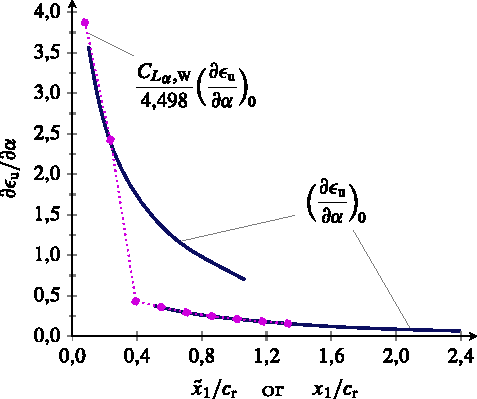
\includegraphics[width=0.65\textwidth]{Chapter_3/aerodynamic_characteristics_of_the_fuselage/fuselage_upwash_close_far_res.pdf}%
  \caption{\finalhyphendemerits=1000
          Gradient of \emph{upwash} at the different stations
           located in front of the wing. The stations named $\tilde{x}_1$ are the closest ones while
            those named $x_1$ these are the stations which are gradually farthest and closest to the bow.
            The two original curves $(\partial\epsilon_\mathrm{u}/\partial\alpha)_0$ are related to a wing of
            lift gradient equal to \SI[round-precision=3]{4.498}{rad^{-1}}. 
           Therefore the desired values are obtained by multiplying by a factor
           $C_{L_\mathlarger{\alpha},\Wing}/\SI[round-precision=3]{4.498}{rad^{-1}}$
           with $C_{L_\mathlarger{\alpha},\Wing}=\SI[round-precision=3]{\myCLAlphaPolhamusWingRAD}{rad^{-1}}$.
  }
  \label{fig:Fuselage:Upwash:Gradient}%
\end{figure}%
%

For the rear trunk of the fuselage we proceed by observing that
\[
\left( 1 + \frac{\partial\epsilon_\mathrm{u}}{\partial\alpha} \right)_\text{\emph{afterbody}}
\simeq
\frac{x_2}{l'_\Htail}\,\left[ 1 - \left(\frac{\partial\epsilon}{\partial\alpha}\right)_{\!\Htail,h_\mathrm{WH}=0} \, \right]
\]
where $\big(\partial\epsilon/\partial\alpha\big)_{\Htail,h_\mathrm{WH=0}}$ is the gradient of \emph{downwash}
at the station $x_2=l'_\Htail$ (coordinate of the aerodynamic center of the tail
horizontal) at the height of the FRL ($Z=0$).
The last formula simply expresses the fact that downstream of the wing the current is diverted downwards
therefore there is an angle of \emph{upwash} $\epsilon_\mathrm{u}$ negative, i.e. a \emph{downwash}
$\epsilon$. Furthermore, it is reasonable to assume that the quantity
\smash{$\big(1+\partial\epsilon_\mathrm{u}/\partial\alpha\big)$}
is almost zero near the trailing edge of the wing ($x_2=0$) and grows
linearly assuming the value \smash{$\big[1-\big(\partial\epsilon/\partial\alpha\big)_{\Htail}\big]$}
at the tail.

In general, to estimate the gradient of \emph{downwash} of the tail
--- at a certain distance downstream of the wing and at a certain height from the wing plane ---
the following analytical formula is used:
\[
%\begin{equation}\label{eq:Aero:Fuselage:Aft:Downwash:Analytic}
%\frac{\diff{\epsilon}}{\diff{\alpha}} 
\left(\frac{\partial\epsilon}{\partial\alpha}\right)_{\!\Htail} =
    \sqrt{1-M^2} \,
    \left[{%
    \num[round-precision=2]{4.44} \bigg( K_{\AR}\,K_{\lambda}\,K_{\Wing\Htail}
        \sqrt{\cos \Lambda_{c/4}}\bigg)^{\num[round-precision=2]{1.19}}\,
    }\right]
%\end{equation}
\]
%valida anche per ali a freccia, 
The multiplying factors
$K_{\AR}$, $K_{\lambda}$ e $K_{\Wing\Htail}$ take into account, respectively,
of the wing aspect ratio $\AR$, wing taper ratio $\lambda$ and of positioning of the plane
of horizontal tail.
They are expressed by the formulas
\[
%\begin{equation}\label{eq:Aero:Fuselage:Aft:Downwash:KAR:Klam:KH}
K_{\AR} = \frac{1}{\AR}-\frac{1}{1+\AR^{\num[round-precision=1]{1.7}}} \;,
\qquad
K_{\lambda} = \frac{10-3\lambda}{7} \;,
\qquad
K_{\Wing\Htail} = \frac{1-\big(h_{\Wing\Htail}/b\big)}{\;\;\,\big(2X_{\Wing\Htail}/b\big)^{1/3}}
  = \frac{1 - \dfrac{m_{\Wing\Htail}}{2}}{r_{\Wing\Htail}^{1/3}}
%\end{equation}
\]
where
% vedi PAMADI
\begin{compactitem}[{\color{gray}$\circ$}]% needs paralist package
\item
$X_{\Wing\Htail}$ is the longitudinal distance, measured in the plane of symmetry
of the aircraft along the direction of the wing root chord,
between point at $\frac{1}{4}$ of the mean aerodynamic chord of the horizontal tail
and point at $\frac{1}{4}$ of the mean aerodynamic chord of the wing,
\item
$h_{\Wing\Htail}$ is the distance from point at $\frac{1}{4}$ of the mean aerodynamic chord of the horizontal tail
from the normal plane to the plane of symmetry of the aircraft
and passing through the root chord of the wing
(conventionally $h_{\Wing\Htail}$is positive if the tailplane is located at
above the root chord).
\end{compactitem}

%
\begin{figure}[t]%[H]%[!htbp]
  %\centering
  %\checkoddpage
  %\centering
    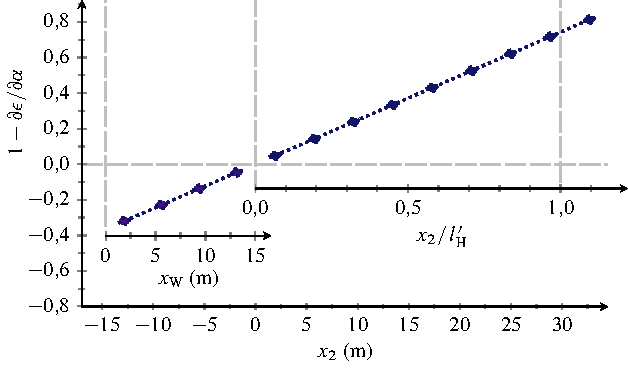
\includegraphics[width=0.80\textwidth]{Chapter_3/aerodynamic_characteristics_of_the_fuselage/fuselage_downwash_wing_afterbody_res.pdf}%
  \caption{\finalhyphendemerits=1000
          Gradient of \emph{downwash} to the different stations
            placed behind the wing. The coordinates $x_\Wing$ and $x_2$ originate, respectively,
            at the leading edge and trailing edge of the wing root chord.
           The length $l'_\Htail$ is the distance of the aerodynamic center of the tail
            horizontal from the origin of the coordinate $x_2$.
  }
  \label{fig:Fuselage:Downwash:Gradient}%
\end{figure}%
%
\EnlargedTableX% needs two latex passes
  {t}% #1: t, b, p
  {%
    \centering
    \begin{tabular}{@{}c@{\rule{6mm}{0pt}}c@{}}
      \emph{forebody strips} & \emph{wing strips} \\
      \adjincludegraphics[valign=T,width=0.42\textwidth]{Chapter_3/aerodynamic_characteristics_of_the_fuselage/fuselage_multhopp_table_2.pdf}%
    &
      \adjincludegraphics[valign=T,width=0.49\textwidth]{Chapter_3/aerodynamic_characteristics_of_the_fuselage/fuselage_multhopp_table_4.pdf}%
    \\
    \multicolumn{2}{c}{%
      \emph{afterbody strips}\rule{0pt}{0.8cm}
    }% end-of-multicolumn
    \\
    \multicolumn{2}{c}{%
      \adjincludegraphics[valign=T,raise=0mm,width=0.42\textwidth]{Chapter_3/aerodynamic_characteristics_of_the_fuselage/fuselage_multhopp_table_3.pdf}%
    }% end-of-multicolumn
    \end{tabular}
    %\vspace{0.3cm}
  }% #2: the image file included by \includegraphics
  {\finalhyphendemerits=1000
    Discretization of the front of the fuselage (\emph{forebody strips}), 
    of the trunk subtended by the wing root (\emph{wing strips}) and the rear part (\emph{afterbody strips}). 
    The numerical values are used in the gradient calculation formula
    \smash{$C_{\mathcal{M}_\mathlarger{\alpha},\Body}$}.
  }% #3: the caption text
  {tab:Fuselage:Multhopp:Results:A:B}%% #4: the label
%
%
\begin{table}[tb]
\caption{%
Summary of the discrete values used in the gradient calculation formula  \smash{$C_{\mathcal{M}_\mathlarger{\alpha},\Body}$}.
 The fuselage discretization is that shown in
  figures~\ref{fig:Fuselage:Sideview:Forebody} and~\ref{fig:Fuselage:Sideview:Afterbody}.
  The three fuselage trunks --- front, center and rear --- are divided, respectively,
   in
  $N_{\mathrm{f}1}=\num[round-precision=0]{\myNoStripForebodyCMAlphaBody}$,
  $N_{\mathrm{f}\Wing}=\num[round-precision=0]{\myNoStripWingCMAlphaBody}$,
  and
  $N_{\mathrm{f}2}=\num[round-precision=0]{\myNoStripAfterbodyCMAlphaBody}$ stripes.
  The strips that count in the calculation of \smash{$C_{\mathcal{M}_\mathlarger{\alpha},\Body}$}
  are those numbered from $1$ to $\num[round-precision=0]{\myNoStripForebodyCMAlphaBody}$
  and from
  \calcSI[round-precision=0,fixed-exponent=0,scientific-notation=fixed]{\myNoStripForebodyCMAlphaBody+\myNoStripWingCMAlphaBody+1}{}
  to
  \calcSI[round-precision=0,fixed-exponent=0,scientific-notation=fixed]{\myNoStripForebodyCMAlphaBody+\myNoStripWingCMAlphaBody+\myNoStripAfterbodyCMAlphaBody}{}.
}
\label{tab:Fuselage:Multhopp:Results:A:C}
\centering
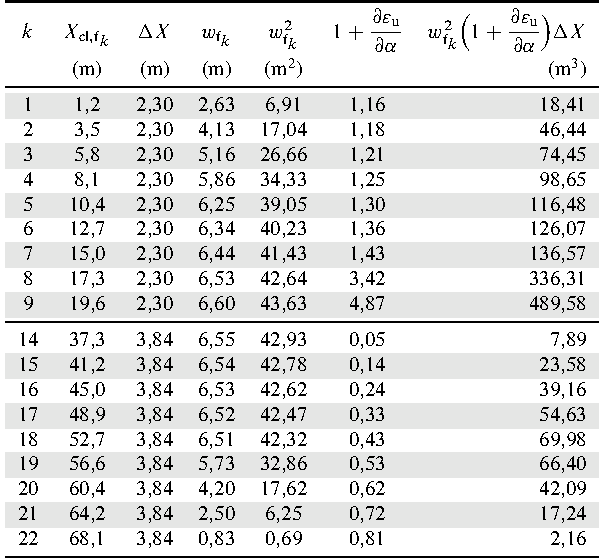
\includegraphics[width=0.68\textwidth]{Chapter_3/aerodynamic_characteristics_of_the_fuselage/fuselage_multhopp_table_5.pdf}
\end{table}
%
In this example it can be assumed for horizontal tail
\[
X_{\Wing\Htail}=\SI[round-precision=1]{\myXrWingMACQuarterChordToHTailMACQuarterChordMT}{m}
  \Longrightarrow
  r_{\Wing\Htail} = \frac{X_{\Wing\Htail}}{b/2}
  = \SI[round-precision=2]{\myFactorRWHDownwashGradientBody}{}
\]

For the purpose of calculating the coefficient \smash{$C_{\mathcal{M}_\mathlarger{\alpha},\Body}$}
it is possible to consider the gradient of \emph{downwash} at the height of the FRL, i.e. for
$h_{\Wing\Htail}=0$. It therefore arises
\[
m_{\Wing\Htail} = 2 \frac{h_{\Wing\Htail}}{b} = \SI[round-precision=0]{0}{}
  \;\Longrightarrow\;
  \left(\frac{\partial\epsilon}{\partial\alpha}\right)_{\!\Htail}
    \equiv \left(\frac{\partial\epsilon}{\partial\alpha}\right)_{\!\Htail,h_{\Wing\Htail}=0}
\]

The three multiplying factors are deduced from the above values
\[
%\begin{equation}\label{eq:Aero:Fuselage:Aft:Downwash:KAR:Klam:KH}
K_{\AR} = \num[round-precision=3]{\myFactorKARDownwashGradientBody}\;,
\qquad
K_{\lambda} = \num[round-precision=2]{\myFactorKlambdaDownwashGradientBody}\;,
\qquad
K_{\Htail} = \num[round-precision=3]{\myFactorKmrDownwashGradientBody}
%\end{equation}
\]
and therefore a
\[
\left(\frac{\partial\epsilon}{\partial\alpha}\right)_{\!\Htail,h_{\Wing\Htail}=0} =
  \mathunderline{mydarkblue}{ 
      \num[round-precision=3]{\myDownwashGradientBody}
  }
\]

The trend of the values of \smash{$\big(\partial\epsilon/\partial\alpha\big)_{\Htail,h_\mathrm{WH=0}}$}
is shown in
figure~\ref{fig:Fuselage:Downwash:Gradient}
and in the table~\ref{tab:Fuselage:Multhopp:Results:A:C}.
%
\begin{figure} [t]%[H]%[!htbp]
  %\centering
  %\checkoddpage
  %\centering
    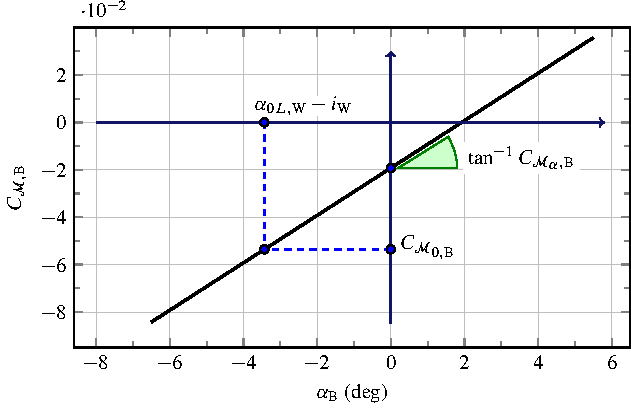
\includegraphics[width=0.70\textwidth]{Chapter_3/aerodynamic_characteristics_of_the_fuselage/fuselage_Cm_vs_alpha.pdf}%
  \caption{\finalhyphendemerits=1000
         Coefficient graph \smash{$C_{\mathcal{M}_\mathlarger{\Body}}$} as the angle of attack changes
         $\alpha_\Body$.
  }
  \label{fig:Fuselage:Cm:Plot}%
\end{figure}%
%
At this point it is possible to decrypt the calculation formula of
\smash{$C_{\mathcal{M}_\mathlarger{\alpha},\Body}$} reaching the following final result:
\[
%\begin{equation}\label{eq:Aero:CMBW:Alpha:Multhopp}
\begin{split}
C_{\mathcal{M}_\mathlarger{\alpha},\Body} 
  % \equiv \bigg(\frac{\partial \CM}{\partial\alpha}\bigg)_{\!\Body(\Wing)} 
  & {}\approx \frac{\pi}{2 S \bar{c}}\, \Bigg(\,
    \sum_{
      k=1
    }^{
      \calcSI[round-precision=0,fixed-exponent=0,scientific-notation=fixed]{\myNoStripForebodyCMAlphaBody}{}
    } w_{\mathrm{f}_\mathlarger{k}}^2 
      \left[ 1 + \left(\frac{\partial \epsilon_\mathrm{u}}{\partial \alpha}\right)_{\!k} \right] \upDelta x_1
    + \sum_{
        k=\calcSI[round-precision=0,fixed-exponent=0,scientific-notation=fixed]{\myNoStripForebodyCMAlphaBody+\myNoStripWingCMAlphaBody+1}{}
      }^{
        \calcSI[round-precision=0,fixed-exponent=0,scientific-notation=fixed]{\myNoStripForebodyCMAlphaBody+\myNoStripWingCMAlphaBody+\myNoStripAfterbodyCMAlphaBody}{}
      } w_{\mathrm{f}_\mathlarger{k}}^2 
      \frac{x_{2_\mathlarger{k}}}{l'_{\mathrm{H}}}
      \left[ 1 - \left(\frac{\partial\epsilon}{\partial\alpha}\right)_{\!\Htail,h_{\Wing\Htail}=0} \right] \upDelta x_2
    \,\Bigg)
\\[4pt]
  &{}= \mathunderline{mydarkblue}{ 
      \SI[round-precision=3]{\myFuselagePitchingMomentCoefficientGradientMulthoppRAD}{rad^{-1}}
  }
  = \mathunderline{mydarkblue}{ 
      \SI[round-precision=4]{\myFuselagePitchingMomentCoefficientGradientMulthoppDEG}{deg^{-1}}
  }
\end{split}
%\end{equation}
\]
The index values $k$ in the previous formula correspond to those reported
in the summary table~\ref{tab:Fuselage:Multhopp:Results:A:C}.

Note the coefficients
\smash{$C_{\mathcal{M}_\mathlarger{0,\Body}}$} and
\smash{$C_{\mathcal{M}_\mathlarger{\alpha},\Body}$}
we can obtai the graph of the \smash{$C_{\mathcal{M}_\mathlarger{\Body}}$}
as a function of the angle $\alpha_\Body$. It corresponds to the line
drawn in the figure~\ref{fig:Fuselage:Cm:Plot}.
Observe the value \smash{$C_{\mathcal{M}_\mathlarger{0,\Body}}$}, for definition,
is associated with the angle $\alpha_\Body=\alpha_{0L,\Wing}-i_\Wing$.

Finally, the displacement, typically forward, of the aerodynamic center is calculated when passing from
wing configuration isolated to the wing-fuselage configuration.
As is known, the extent of the shift is given by the ratio
\[
-\frac{C_{\mathcal{M}_\mathlarger{\alpha},\Body} }{ C_{L_\mathlarger{\alpha},\Wing} }
  \equiv \upDelta \bar{x}_{\mathrm{ac},\Wing\rightarrow\Wing\Body}
  = - \frac{
      \SI[round-precision=3]{\myFuselagePitchingMomentCoefficientGradientMulthoppRAD}{rad^{-1}}
    }{
      \SI[round-precision=2]{\myCLAlphaPolhamusWingRAD}{rad^{-1}}
    }
  = \mathunderline{mydarkblue}{ 
    - \calcSI[round-precision=3,fixed-exponent=0,scientific-notation=fixed]{
      \myFuselagePitchingMomentCoefficientGradientMulthoppRAD / \myCLAlphaPolhamusWingRAD
      }{}
  }
\]
Note the distance from the leading edge of the medium aerodynamic chord of the isolated wing,
which in the analyzed case is $x_{\mathrm{ac},\Wing}\,\bar{c} = \SI[round-precision=3]{\myXsiACWing}{}\,\bar{c}$,
the dimensionless position of the aerodynamic center
of the partial aircraft is therefore:
\[
\bar{x}_{\mathrm{ac},\Wing\Body}
  \equiv \frac{x_{\mathrm{ac},\Wing\Body}}{\bar{c}}
  = \frac{x_{\mathrm{ac},\Wing}}{\bar{c}} - \frac{C_{\mathcal{M}_\mathlarger{\alpha},\Body}}{C_{L_\mathlarger{\alpha},\Wing}}
%
  = \SI[round-precision=3]{\myXsiACWing}{}
  - \calcSI[round-precision=3,fixed-exponent=0,scientific-notation=fixed]{
    \myFuselagePitchingMomentCoefficientGradientMulthoppRAD / \myCLAlphaPolhamusWingRAD
    }{}
%
  = \mathunderline{mydarkblue}{ \SI[round-precision=3]{\myXsiACWingBodyMulthopp}{} }
\]
%
The distances $x_{\mathrm{ac},\Wing}$ and $x_{\mathrm{ac},\Wing\Body}$ for 
% l'esempio di calcolo 
the aircraft
considered are shown
in the figure~\ref{fig:Fuselage:Multhopp:Results:A:CA:Shift}.
%
\EnlargedFigureX% needs two latex passes
  {t}% #1: t, b, p
  {%
    \makebox[\textwidth][c]{%
      \rule{2.2mm}{0pt}% --> hack
      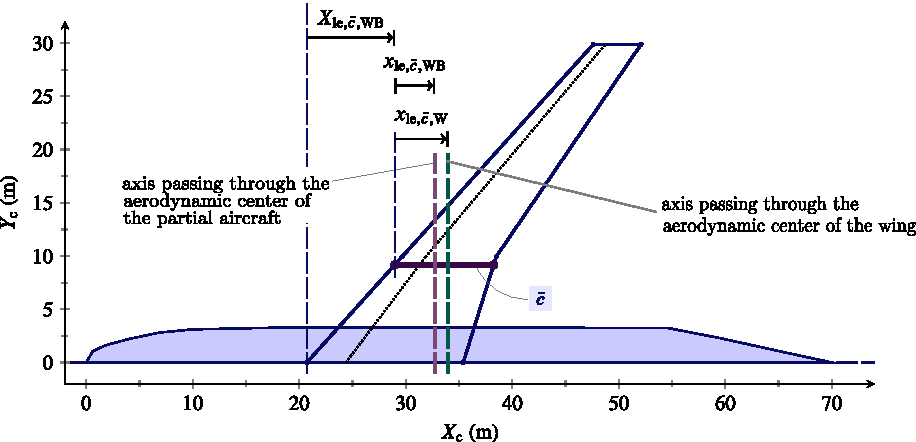
\includegraphics[width=0.90\textwidth]{Chapter_3/aerodynamic_characteristics_of_the_fuselage/fuselage_topview_2.pdf}%
    }% end-of-makebox
    %\vspace{0.3cm}
  }% #2: the image file included by \includegraphics
  {\finalhyphendemerits=1000
    Effect of the presence of the fuselage on the aerodynamic center.
   For clarity the coordinates have been highlighted $(X_\mathrm{c},Y_\mathrm{c})$ of the reference system \emph{constructive}
    of the aircraft, using the symbol `$X$'for the longitudinal distances referred to the apex of the wing
    is `$x$' for those referring to the leading edge of the medium aerodynamic rope.
     The aerodynamic center of the wing, in the transition to the wing-fuselage configuration,
     typically moves forward.
     In the example proposed, we pass by a value 
    $x_{\mathrm{ac},\Wing}/{\bar{c}}=\SI[round-precision=3]{\myXsiACWing}{}$
    to a value
    $x_{\mathrm{ac},\Wing\Body}/{\bar{c}}=\SI[round-precision=3]{\myXsiACWingBodyMulthopp}{}$.
  }% #3: the caption text
  {fig:Fuselage:Multhopp:Results:A:CA:Shift}%% #4: the label
%
\end{myExampleX}
\end{document}